\chapter{Лабораторная работа №4 \\
Расчёт и моделирование направленного ответвителя на связанных линиях}

Цель работы: ознакомиться с расчётом и моделированием направленного ответвителя на связанных линиях в среде Keysight Advanced Design System (ADS).

Используемое оборудование или ПО: Keysight Advanced Design System 2020 upd1.

\section{Техническое задание}

Рассчитать и спроектировать направленный ответвитель на связанных линиях на входную частоту $F_c = 7 \text{~ГГц}$, обеспечив переходное ослабление в $k = 15 \text{~дБ}$.
Провести её настройку и исследование на схемном и топологическом уровнях.

В качестве подложки использовать Arlon AD255C с относительной диэлектрической проницаемостью $\epsilon = 2.55$, тангенсом угла диэлектрических потерь $\tg{\delta} = 0.0013$, толщиной диэлектрика $H = 0.508 \text{~мм}$ и толщиной металлизации $T = 35 \text{~мкм}$.

\section{Выполнение работы}

\subsection{Создание подложки}

В первую очередь зададим параметры подложки.

Для этого в главном окне перейдём по пути Options\textrightarrow Technology\textrightarrow Edit Stackup (tech.subst) и выберем пункт Create the master substrate from scratch.
В качестве шаблона используем 25milAlumina.
Параметры подложки возьмём из технического задания.

Результат представлен на рис. \ref{fig:directional_coupler_substrate}.

\begin{figure}
    \centering
    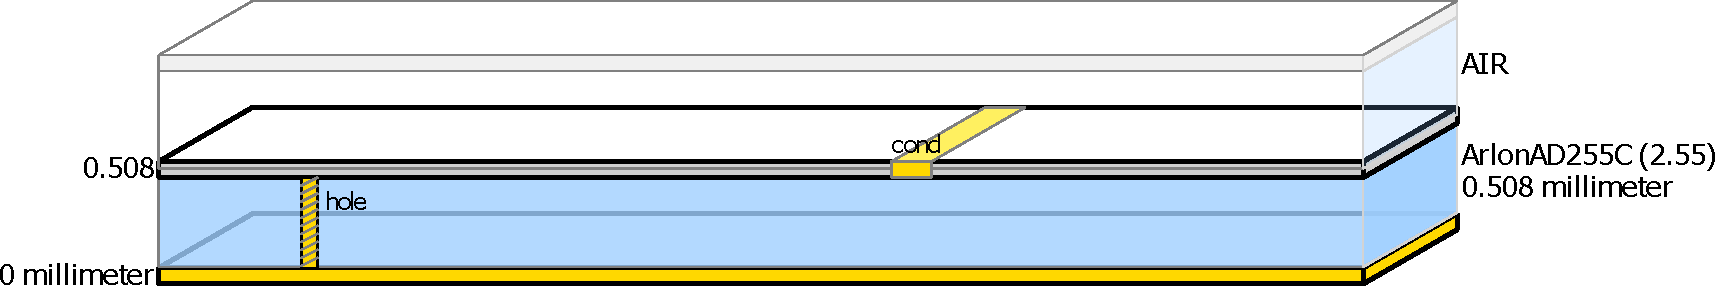
\includegraphics[width=0.9\textwidth]{directional_coupler_substrate.pdf}
    \caption{Подложка}
    \label{fig:directional_coupler_substrate}
\end{figure}

\subsection{Модель на идеальных линиях передачи}

Соберём моделируемую схему на идеальных линиях передачи (Рис. \ref{fig:directional_coupler_ideal_schematic}).

\begin{figure}[!ht]
    \centering
    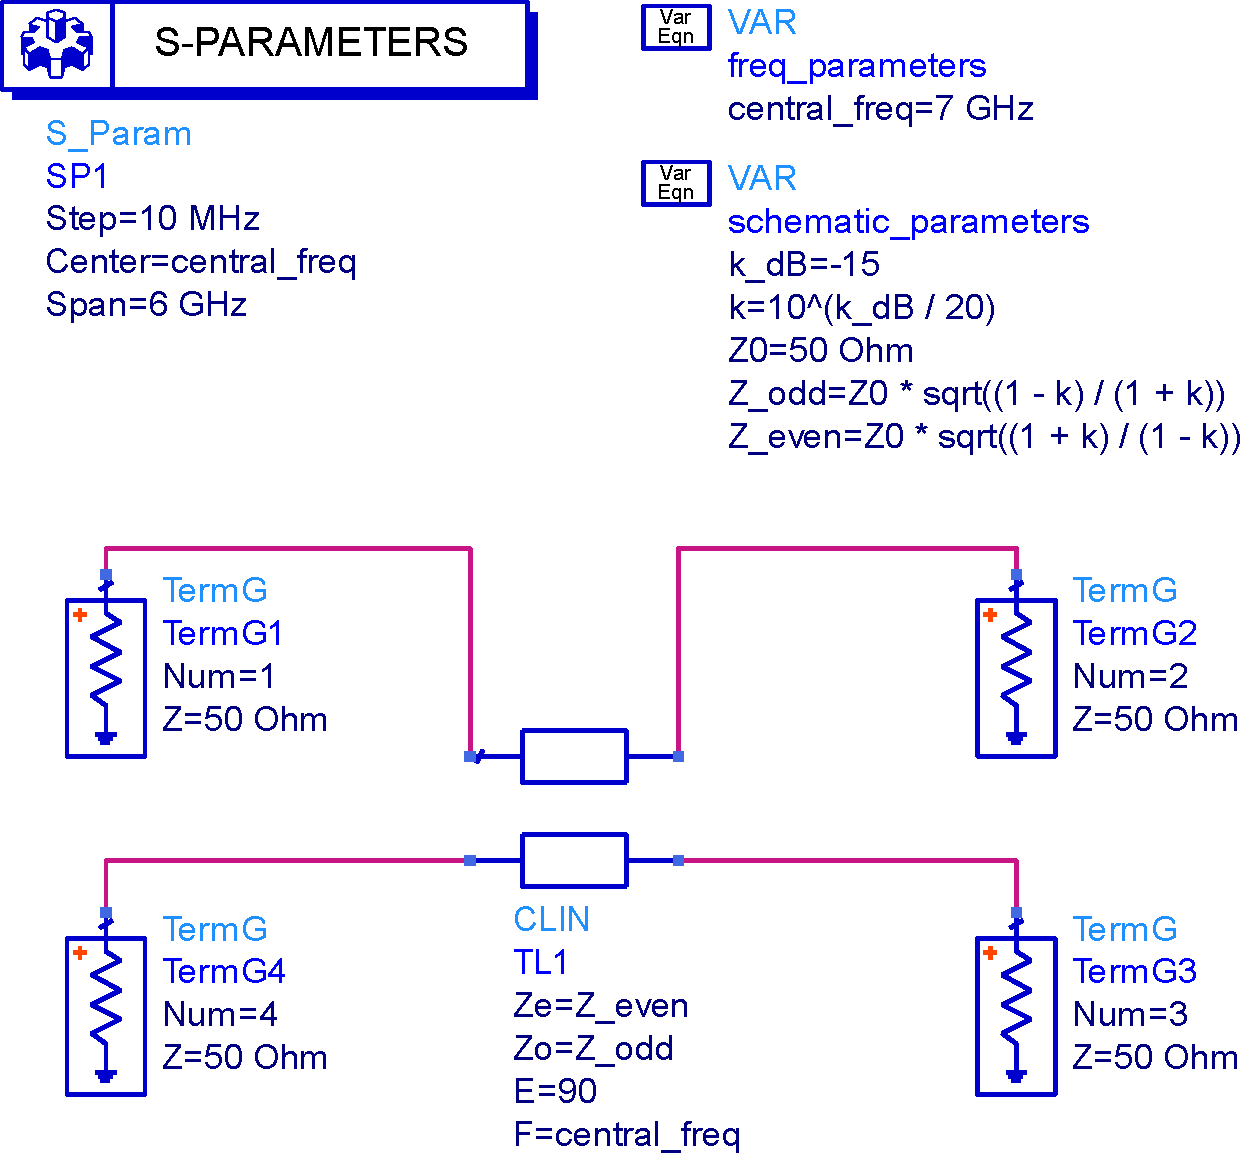
\includegraphics[width=0.8\textwidth]{directional_coupler_ideal_schematic.pdf}
    \caption{Моделируемая цепь на идеальных линиях передачи}
    \label{fig:directional_coupler_ideal_schematic}
\end{figure}

Результаты моделирования можно увидеть на рис. \ref{fig:directional_coupler_ideal_data_1}.

\begin{figure}[!ht]
    \centering
    \begin{subfigure}[b]{0.40\textwidth}
        \centering
        \includegraphics[width=\textwidth]{directional_coupler_ideal_data_1_in1_freq_response.pdf}
        \caption{}
        \label{fig:directional_coupler_ideal_data_1_in1_freq_response}
    \end{subfigure}
    \hfill
    \begin{subfigure}[b]{0.40\textwidth}
        \centering
        \includegraphics[width=\textwidth]{directional_coupler_ideal_data_1_in1_phase_response.pdf}
        \caption{}
        \label{fig:directional_coupler_ideal_data_1_in1_phase_response}
    \end{subfigure}
    \caption{
        a) АЧХ моделируемой цепи по первому входу;
        б) ФЧХ моделируемой цепи по первому входу
    }
    \label{fig:directional_coupler_ideal_data_1_in1}
\end{figure}

\begin{figure}[!ht]
    \begin{subfigure}[b]{0.40\textwidth}
        \centering
        \includegraphics[width=\textwidth]{directional_coupler_ideal_data_1_in3_freq_response.pdf}
        \caption{}
        \label{fig:directional_coupler_ideal_data_1_in3_freq_response}
    \end{subfigure}
    \hfill
    \begin{subfigure}[b]{0.40\textwidth}
        \centering
        \includegraphics[width=\textwidth]{directional_coupler_ideal_data_1_in3_phase_response.pdf}
        \caption{}
        \label{fig:directional_coupler_ideal_data_1_in3_phase_response}
    \end{subfigure}
    \caption{
        а) АЧХ моделируемой цепи по третьему входу;
        б) ФЧХ моделируемой цепи по третьему входу
    }
    \label{fig:directional_coupler_ideal_data_1_in3}
\end{figure}

Оценим симметричность сигналов. Для этого зададим рассчитывающие их выражения и выведем АЧХ и ФЧХ этого соотношения (Рис. \ref{fig:directional_coupler_ideal_data_1_ripple_responses}).

\begin{figure}[!ht]
    \centering
    \begin{subfigure}[b]{\textwidth}
        \centering
        \includegraphics[width=0.3\textwidth]{directional_coupler_ideal_data_1_ripple_equations.pdf}
        \caption{}
        \label{fig:directional_coupler_ideal_ripple_equations}
    \end{subfigure}
    \vfill
    \begin{subfigure}[b]{0.45\textwidth}
        \centering
        \includegraphics[width=\textwidth]{directional_coupler_ideal_data_1_ripple_freq_response.pdf}
        \caption{}
        \label{fig:directional_coupler_ideal_data_1_ripple_freq_response}
    \end{subfigure}
    \hfill
    \begin{subfigure}[b]{0.45\textwidth}
        \centering
        \includegraphics[width=\textwidth]{directional_coupler_ideal_data_1_ripple_phase_response.pdf}
        \caption{}
        \label{fig:directional_coupler_ideal_data_1_ripple_phase_response}
    \end{subfigure}
    \caption{
        a) Выражения для рассчёта ассиметричности;
        б) АЧХ ассиметричности;
        в) ФЧХ ассиметричности
    }
    \label{fig:directional_coupler_ideal_data_1_ripple_responses}
\end{figure}

В этом же окне выведеи идеальную теоретическую матрицу рассеяния (Рис. \ref{fig:directional_coupler_ideal_data_1_smatrix}).
\begin{figure}[!ht]
    \centering
    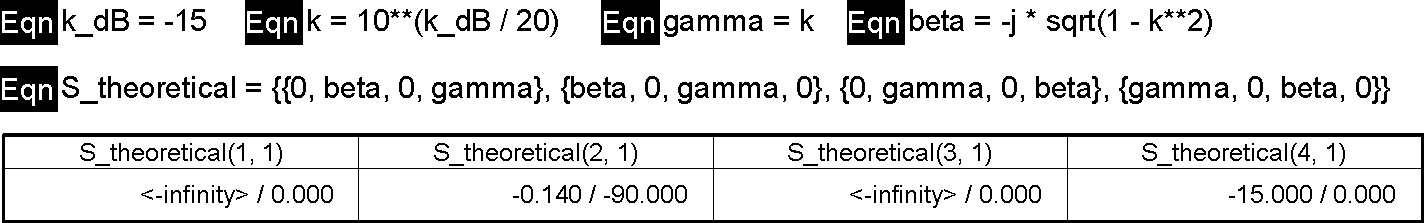
\includegraphics[width=0.8\textwidth]{directional_coupler_ideal_data_1_smatrix}
    \caption{Идеальная теоретическая матрица рассеяния}
    \label{fig:directional_coupler_ideal_data_1_smatrix}
\end{figure}
Коэффициенты отражения $S_{11}$ и $S_{33}$, а также развязка $S_{31}$ имеют значение по амплитуде $-\infty \text{~дБ}$. Рабочие затухания $S_{21}$ и $S_{32}$ и переходные ослабления $S_{41}$ и $S_{41}$ равны $-3 \text{~дБ}$. По фазовым соотношениям видны суммарный и разностный выходы.

Дополнительно рассчитаем и выведем волновые сопротивления участков относительно $Z_0 = 50 \text{~Ом}$ (Рис. \ref{fig:directional_coupler_ideal_data_1_impedances_and_admittances}).
\begin{figure}[!ht]
    \centering
    \includegraphics[width=0.6\textwidth]{directional_coupler_ideal_data_1_impedances_and_admittances.pdf}
    \caption{Волновые сопротивления и проводимости}
    \label{fig:directional_coupler_ideal_data_1_impedances_and_admittances}
\end{figure}

\subsection{Модель на схемном уровне в микрополосковом исполнении}

Для расчёта геометрических размеров нескольких видов линий передач воспользуемся инструментом LineCalc, которую можно найти по пути Tools\textrightarrow LineCalc\textrightarrow Start LineCalc.

В подокне Substrate Parameters задаём параметры подложки из технического задания, в подокне Component Parameters задаём частоту из технического задания, а в подокне Electrical "--- импеданс и электрическую длину, для которых ведётся расчёт.
После этого, нажав кнопку Synthesize, получим в подокне Physical искомые геометрические размеры.

Расчитаем таким образом геометрические размеры дуг.
Получим $W_{50} = 1.383 \text{~мм}$ и $W_{71} = 0.756 \text{~мм}$, $L_\text{curve} = 7.370 \text{~мм}$ соответственно.

Построим моделируемую схему в микрополосковом исполнении (Рис. \ref{fig:directional_coupler_MLIN_schematic_1}).

\begin{figure}[!ht]
    \centering
    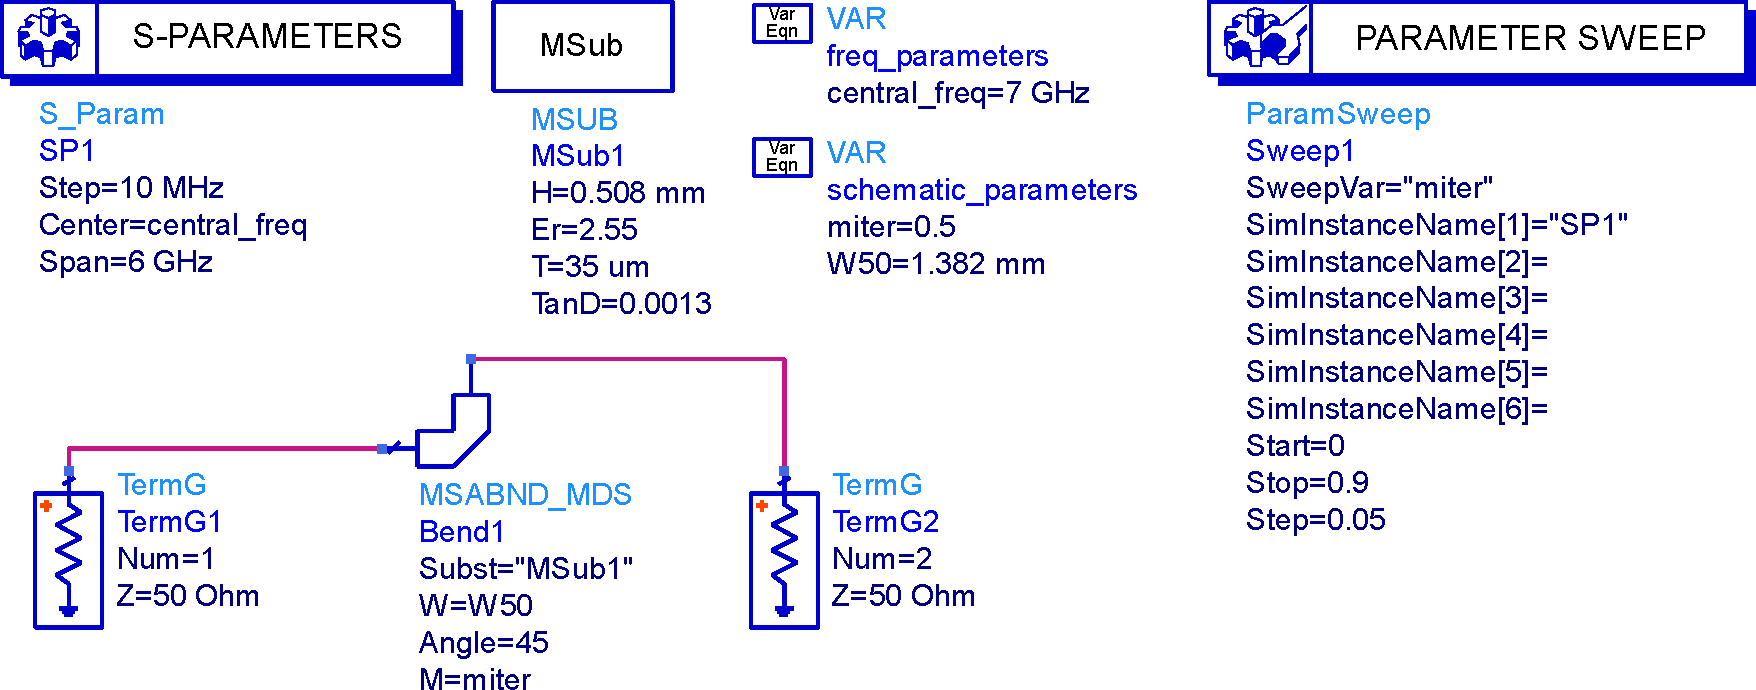
\includegraphics[width=0.8\textwidth]{directional_coupler_MLIN_schematic_1.pdf}
    \caption{Моделируемая схема в микрополосковом исполнении}
    \label{fig:directional_coupler_MLIN_schematic_1}
\end{figure}

Запустим расчёт и выведем АЧХ (Рис. \ref{fig:directional_coupler_MLIN_data_1_freq_response}).

\begin{figure}[!ht]
    \begin{subfigure}[b]{0.45\textwidth}
        \centering
        \includegraphics[width=\textwidth]{directional_coupler_MLIN_data_1_in1_freq_response.pdf}
        \caption{}
        \label{fig:directional_coupler_MLIN_data_1_in1_freq_response}
    \end{subfigure}
    \hfill
    \begin{subfigure}[b]{0.45\textwidth}
        \centering
        \includegraphics[width=\textwidth]{directional_coupler_MLIN_data_1_in3_freq_response.pdf}
        \caption{}
        \label{fig:directional_coupler_MLIN_data_1_in3_freq_response}
    \end{subfigure}
    \caption{АЧХ моделируемой схемы в микрополосковом исполнении:
        а) по первому входу;
        б) по третьему входу
    }
    \label{fig:directional_coupler_data_1_freq_response}
\end{figure}

Результаты показывают, что рабочая частота устройства уплыла вниз. Связано это с добавлением на схему тройников и компенсирующих их участков, в результате чего электрические длины дуг оказались больше, чем требуется.
Для того, чтобы исправить это, воспользуемся инструментом Tune.
В качестве изменяемого параметра укажем $L_\text{curve}$, для чего щёлкнем по нему левой кнопкой мыши.
Подберём оптимальный размер шага, после чего изменяя значения выбранного параметра с помощью слайдера, найдём такое, при котором обеспечивается наилучшее согласование.
В дополнение к этому поставим следующие условия:
\begin{itemize}
    \item коэффициенты отражения $dB(S_{11})$ и $dB(S_{33})$ и развязка $dB(S_{31})$ не должны превышать $-25 \text{~дБ}$ в диапазоне $(6.6 .. 7.4) \text{~ГГц}$;
    \item положение провалов коэффициентов отражения $dB(S_{11})$ $dB(S_{33})$ и развязки $dB(S_{31})$ как можно ближе к $7 \text{~ГГц}$;
    \item рабочие затухания $dB(S_{21})$ и $dB(S_{32})$ и переходные ослабления $dB(S_{41})$ и $dB(S_{43})$ не должны опускаться ниже $-3.5 \text{~дБ}$;
\end{itemize}
Для переноса получившихся значений на схему нажмём кнопку Update Schematic в окне Tune Parameters.

Итоговую схему можем увидеть на рис. \ref{fig:directional_coupler_MLIN_schematic_2}, а её характеристики приобретут вид как на рис. \ref{fig:directional_coupler_MLIN_data_2}.

\begin{figure}
    \centering
    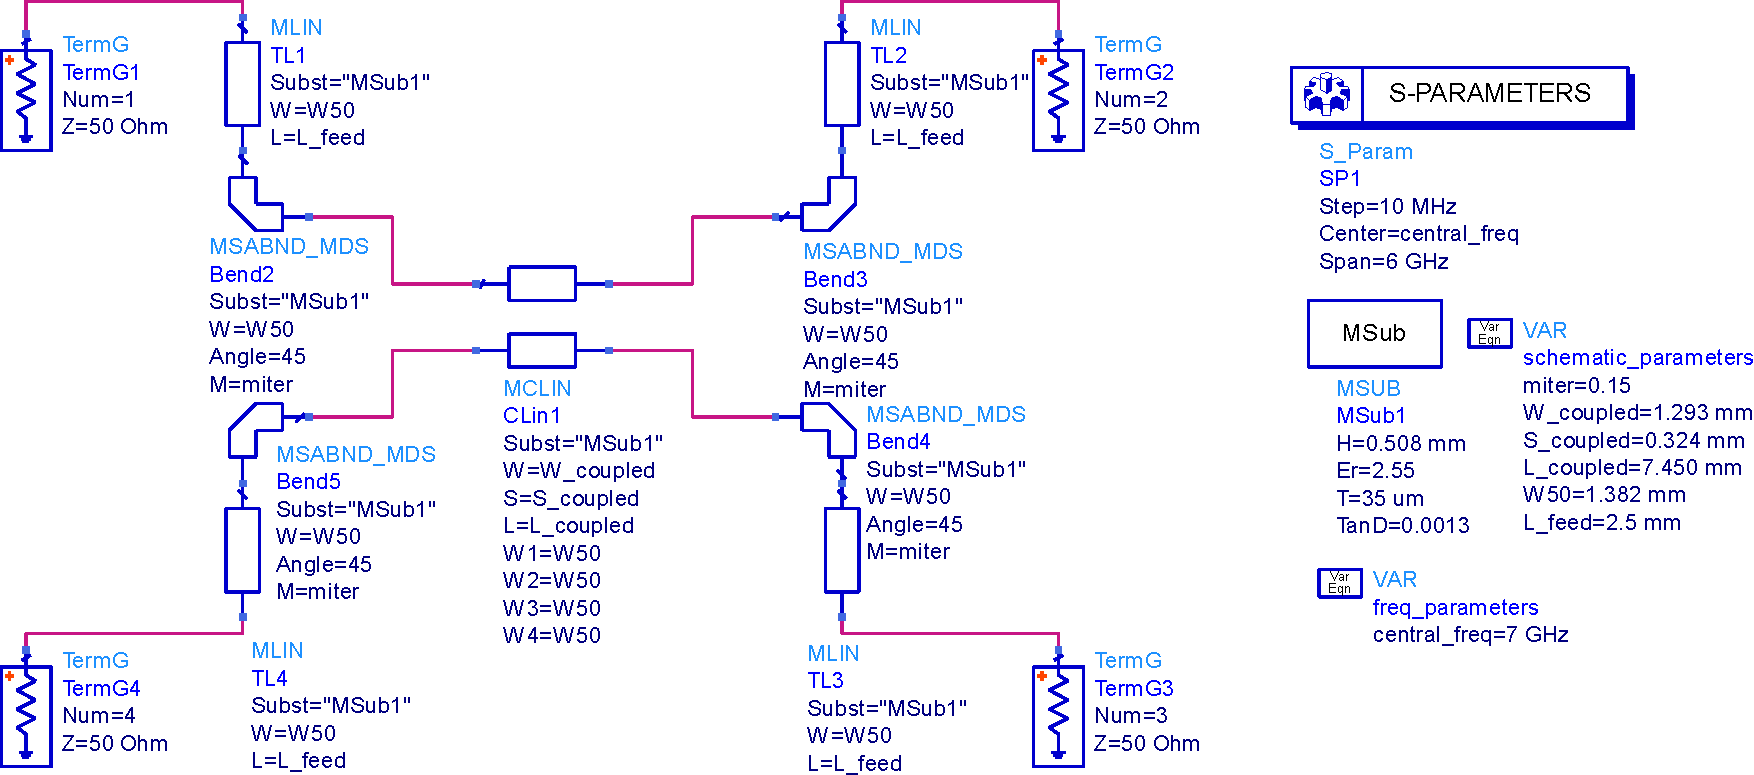
\includegraphics[width=0.6\textwidth]{directional_coupler_MLIN_schematic_2.pdf}
    \caption{Моделируемая схема в микрополосковом исполнении после применения инструмента Tune}
    \label{fig:directional_coupler_MLIN_schematic_2}
\end{figure}

\begin{figure}[!ht]
    \centering
    \begin{subfigure}[b]{0.45\textwidth}
        \centering
        \includegraphics[width=\textwidth]{directional_coupler_MLIN_data_2_in1_freq_response.pdf}
        \caption{}
        \label{fig:directional_coupler_MLIN_data_2_in1_freq_response}
    \end{subfigure}
    \hfill
    \begin{subfigure}[b]{0.45\textwidth}
        \centering
        \includegraphics[width=\textwidth]{directional_coupler_MLIN_data_2_in3_freq_response.pdf}
        \caption{}
        \label{fig:directional_coupler_MLIN_data_2_in3_freq_response}
    \end{subfigure}
    \caption{
        Частотные характеристики моделируемой схемы в микрополосковом исполнении после применения инструмента Tune:
        a) АЧХ по первому входу;
        б) АЧХ по третьему входу
    }
    \label{fig:directional_coupler_MLIN_data_2}
\end{figure}

Неравномерность частотных характеристик в заданном диапазоне можно увидеть на рис. \ref{fig:directional_coupler_MLIN_data_2_response_ripple}.

\begin{figure}[!ht]
    \centering
    \begin{subfigure}[b]{0.4\textwidth}
        \centering
        \includegraphics[width=\textwidth]{directional_coupler_MLIN_data_2_ripple_equations.pdf}
        \caption{}
        \label{fig:directional_coupler_MLIN_data_2_ripple_equations}
    \end{subfigure}
    \vfill
    \begin{subfigure}[b]{0.40\textwidth}
        \centering
        \includegraphics[width=\textwidth]{directional_coupler_MLIN_data_2_ripple_freq_response.pdf}
        \caption{}
        \label{fig:directional_coupler_MLIN_data_2_ripple_freq_response}
    \end{subfigure}
    \hfill
    \begin{subfigure}[b]{0.50\textwidth}
        \centering
        \includegraphics[width=\textwidth]{directional_coupler_MLIN_data_2_ripple_phase_response.pdf}
        \caption{}
        \label{fig:directional_coupler_MLIN_data_2_ripple_phase_response}
    \end{subfigure}
    \caption{
        Неравномерность рабочего затухания и переходного ослабления:
        а) выражения для рассчёта;
        б) АЧХ;
        в) ФЧХ
    }
    \label{fig:directional_coupler_MLIN_data_2_response_ripple}
\end{figure}

\subsection{Модель на топологическом уровне}

Скопируем схему в микрополосковом исполнении в новую ячейку. Сделаем её двухуровневой, перенеся во внутренний уровень все полосковые устройства. Сделать это можно по команде Edit\textrightarrow Component\textrightarrow Create Hierarchy.

В результате получим схему верхнего уровня (Рис. \ref{fig:directional_coupler_EM_schematic}) и схему нижнего уровня (Рис. \ref{fig:directional_coupler_EM_inner_schematic}).

\begin{figure}[!ht]
    \centering
    \begin{subfigure}[b]{0.45\textwidth}
        \centering
        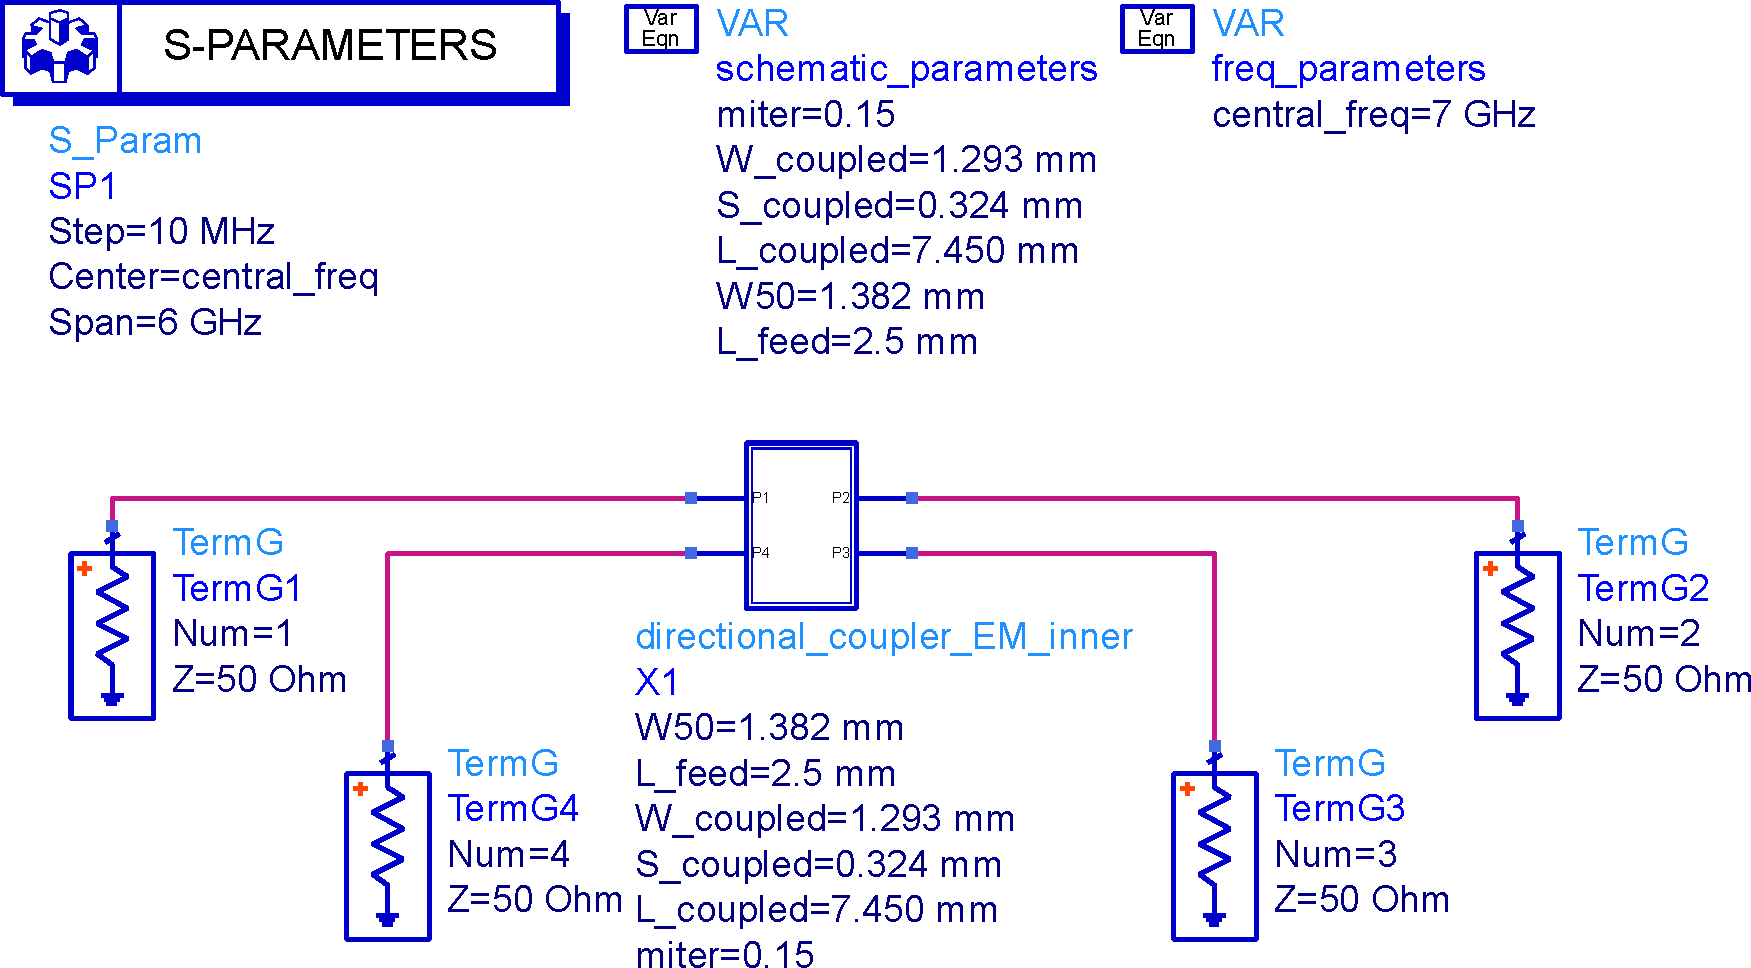
\includegraphics[width=\textwidth]{directional_coupler_EM_schematic_1.pdf}
        \caption{}
        \label{fig:directional_coupler_EM_schematic}
    \end{subfigure}
    \hfill
    \begin{subfigure}[b]{0.45\textwidth}
        \centering
        \includegraphics[width=\textwidth]{directional_coupler_EM_inner_schematic_1.pdf}
        \caption{}
        \label{fig:directional_coupler_EM_inner_schematic}
    \end{subfigure}
    \caption{
        Моделируемая схема на топологическом уровне:
        a) внешнаяя схема;
        б) внутренняя схема
    }
    \label{fig:directional_coupler_EM_schematics}
\end{figure}

Перейдём в схему нижнего уровня. Для получения топологического представления воспользуемся функцией Layout\textrightarrow Generate/Update Layout.
Топологическое представление создано верно (Рис. \ref{fig:directional_coupler_layout_check}).

\begin{wrapfigure}{l}{0.4\textwidth}
    \centering
    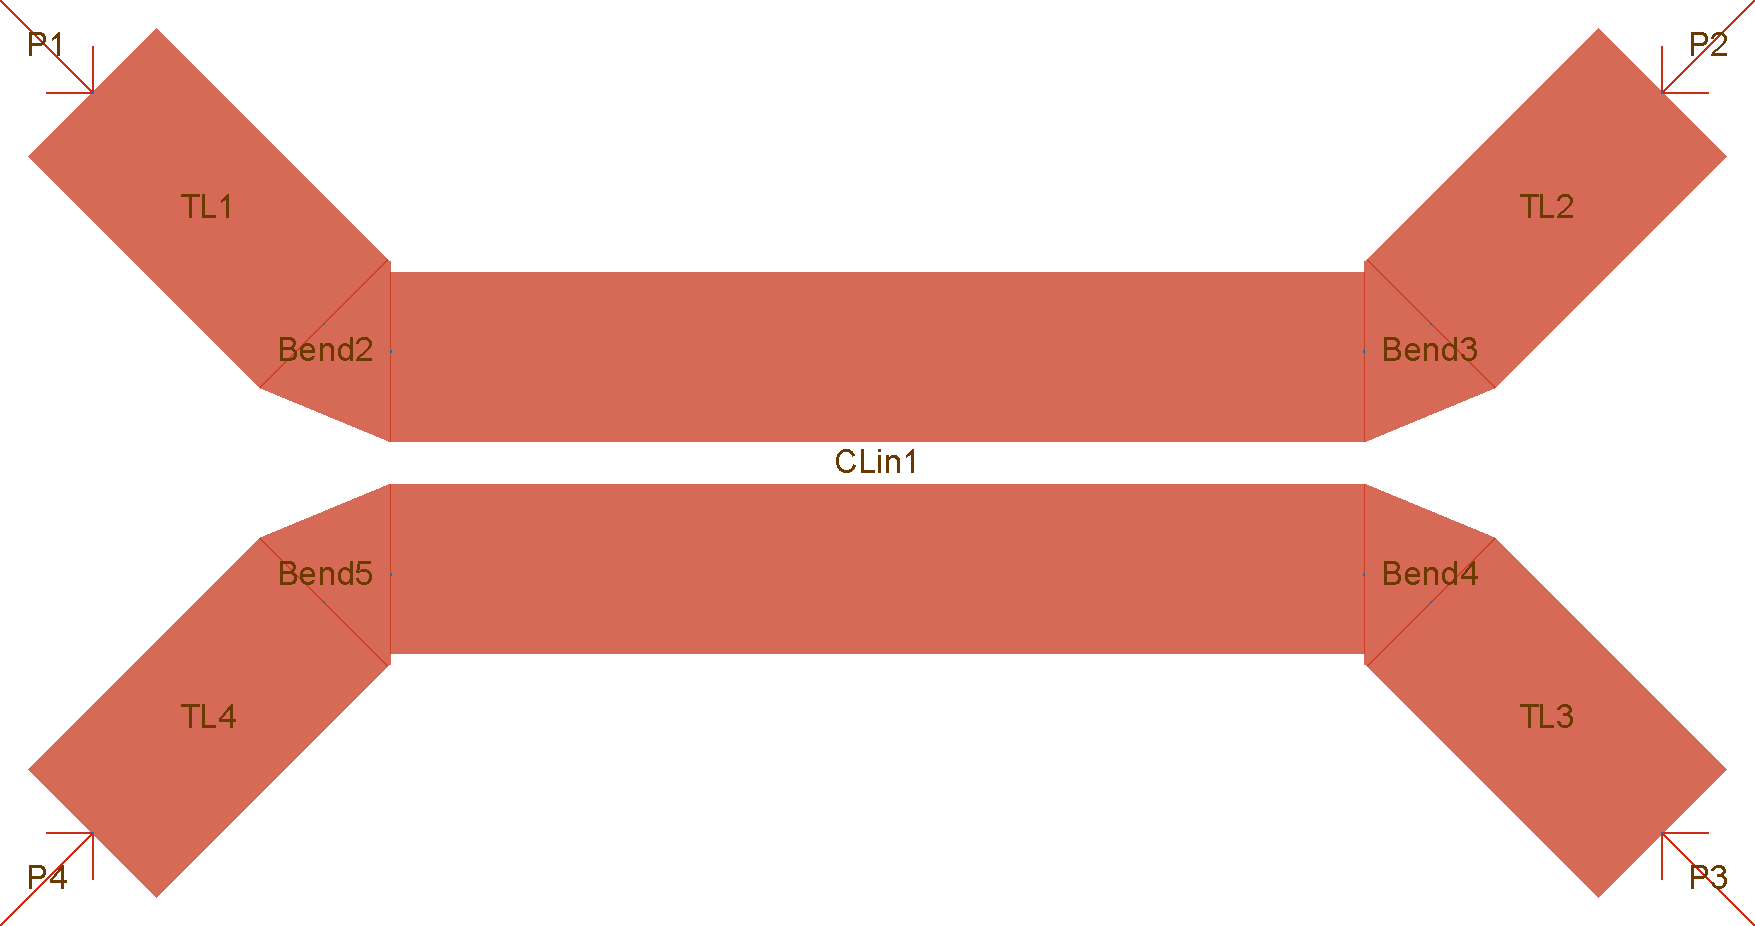
\includegraphics[width=0.4\textwidth]{directional_coupler_layout_check.pdf}
    \caption{Проверка топологического представления}
    \label{fig:directional_coupler_layout_check}
\end{wrapfigure}

Перейдём в окно File\textrightarrow Customize Pcell.
Сделаем схему параметризуемой, выбрав в выпадающем списке тип Parameterized sub network Pcell.
Также убедимся в том, что выставлены галочки напротив Support non-90 degree rotation и Support unit and database resolution for ADS 2015 and older.

В окне File\textrightarrow Cell Parameters определим параметры $W_{50}$, $L_\text{feed}$, $L_\text{shunt}$, $L_\text{serial}$.

Для EM-моделирования создадим сущность emSetup.
Это можно сделать в окне EM\textrightarrow Simulation Setting.
Определим параметры в соответствии с требованиями.

Запустим моделирование S-параметров нажатием кнопки Simulate.
В результате на топологии появится сетка (Рис. \ref{fig:directional_coupler_layout_sparam}).

\begin{wrapfigure}{r}{0.4\textwidth}
    \centering
    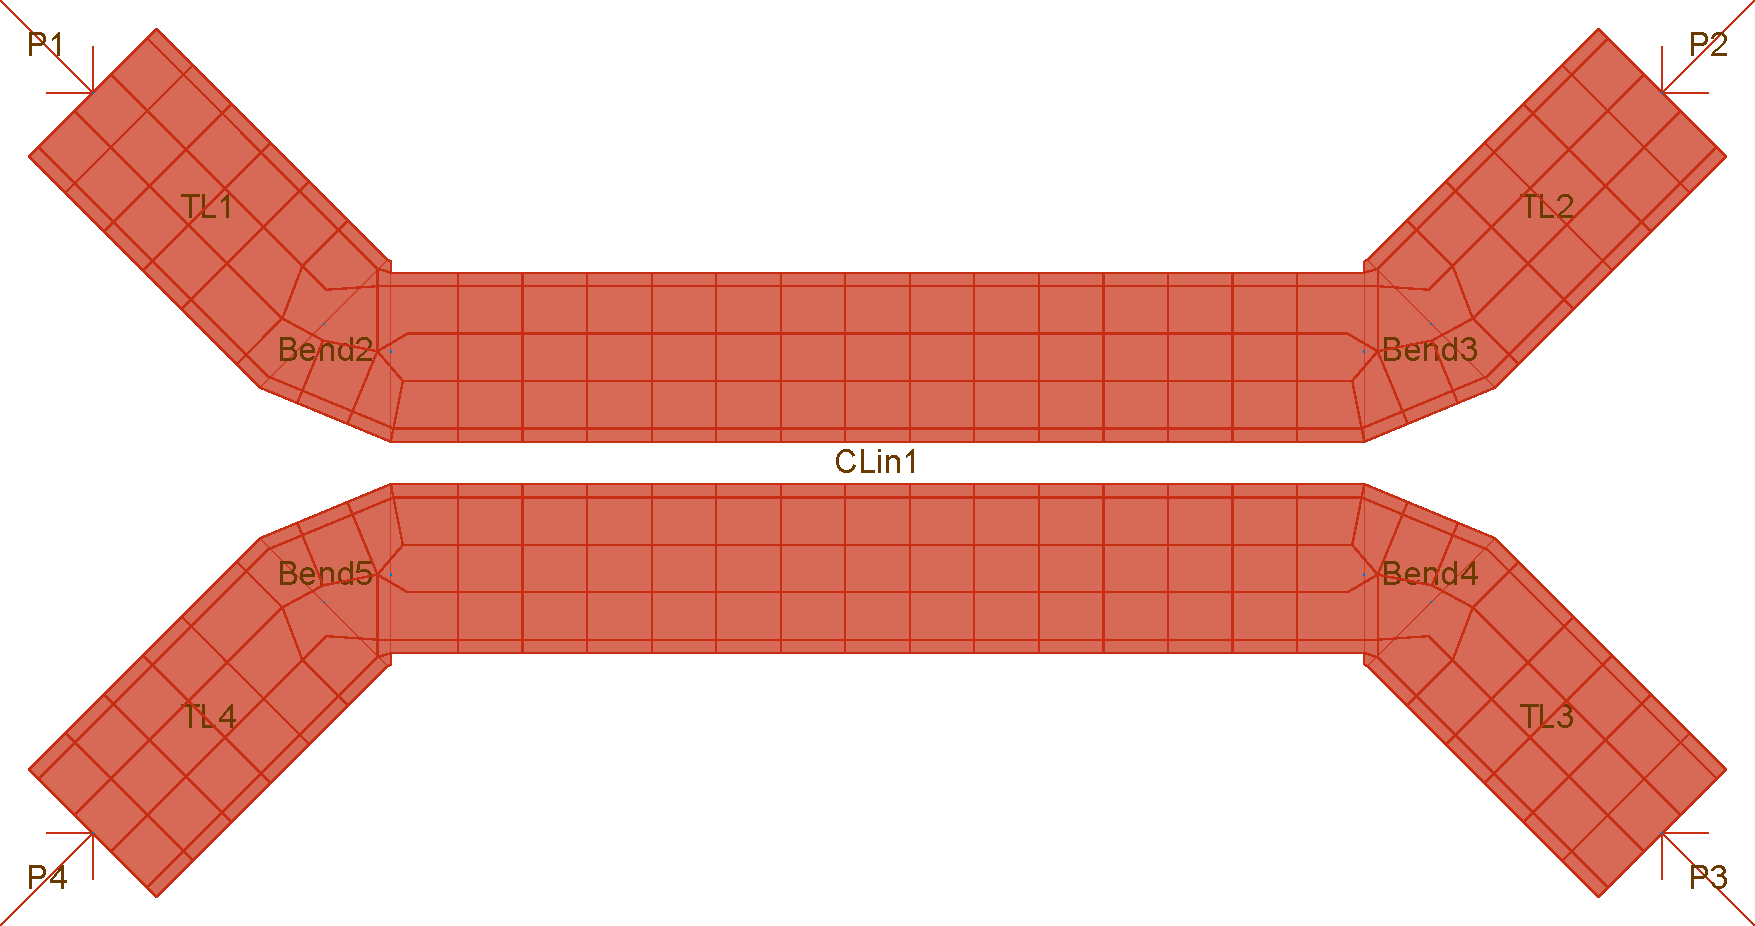
\includegraphics[width=0.4\textwidth]{directional_coupler_layout_sparam.pdf}
    \caption{Сетка на топологическом представлении после проведения EM-моделирования}
    \label{fig:directional_coupler_layout_sparam}
\end{wrapfigure}

Из окна emSetup можно обновить отображение элемента на схеме.
Сделаем так, чтоб оно подгружалось из топологии (Рис. \ref{fig:directional_coupler_symbol}).

\begin{wrapfigure}{l}{0.4\textwidth}
    \centering
    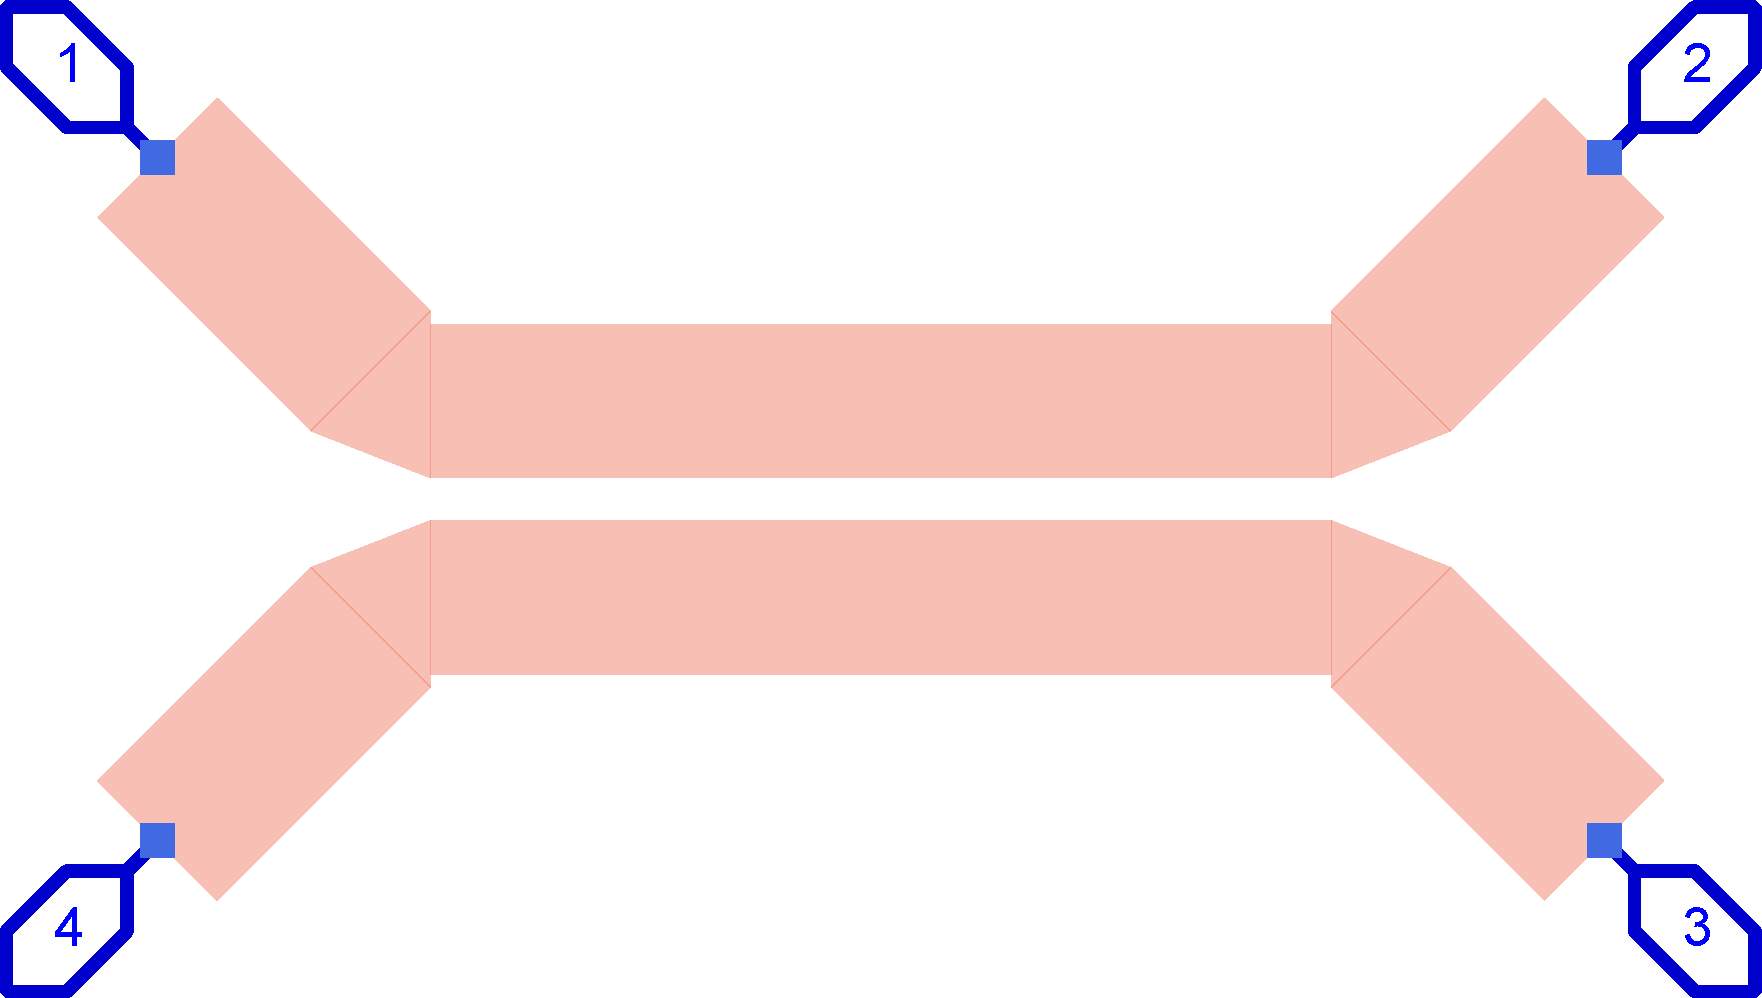
\includegraphics[width=0.4\textwidth]{directional_coupler_symbol.pdf}
    \caption{Обновлённый символ}
    \label{fig:directional_coupler_symbol}
\end{wrapfigure}

В итоге схема приобретёт вид как на рис. \ref{fig:directional_coupler_EM_schematic_2}.

\begin{figure}[p]
    \centering
    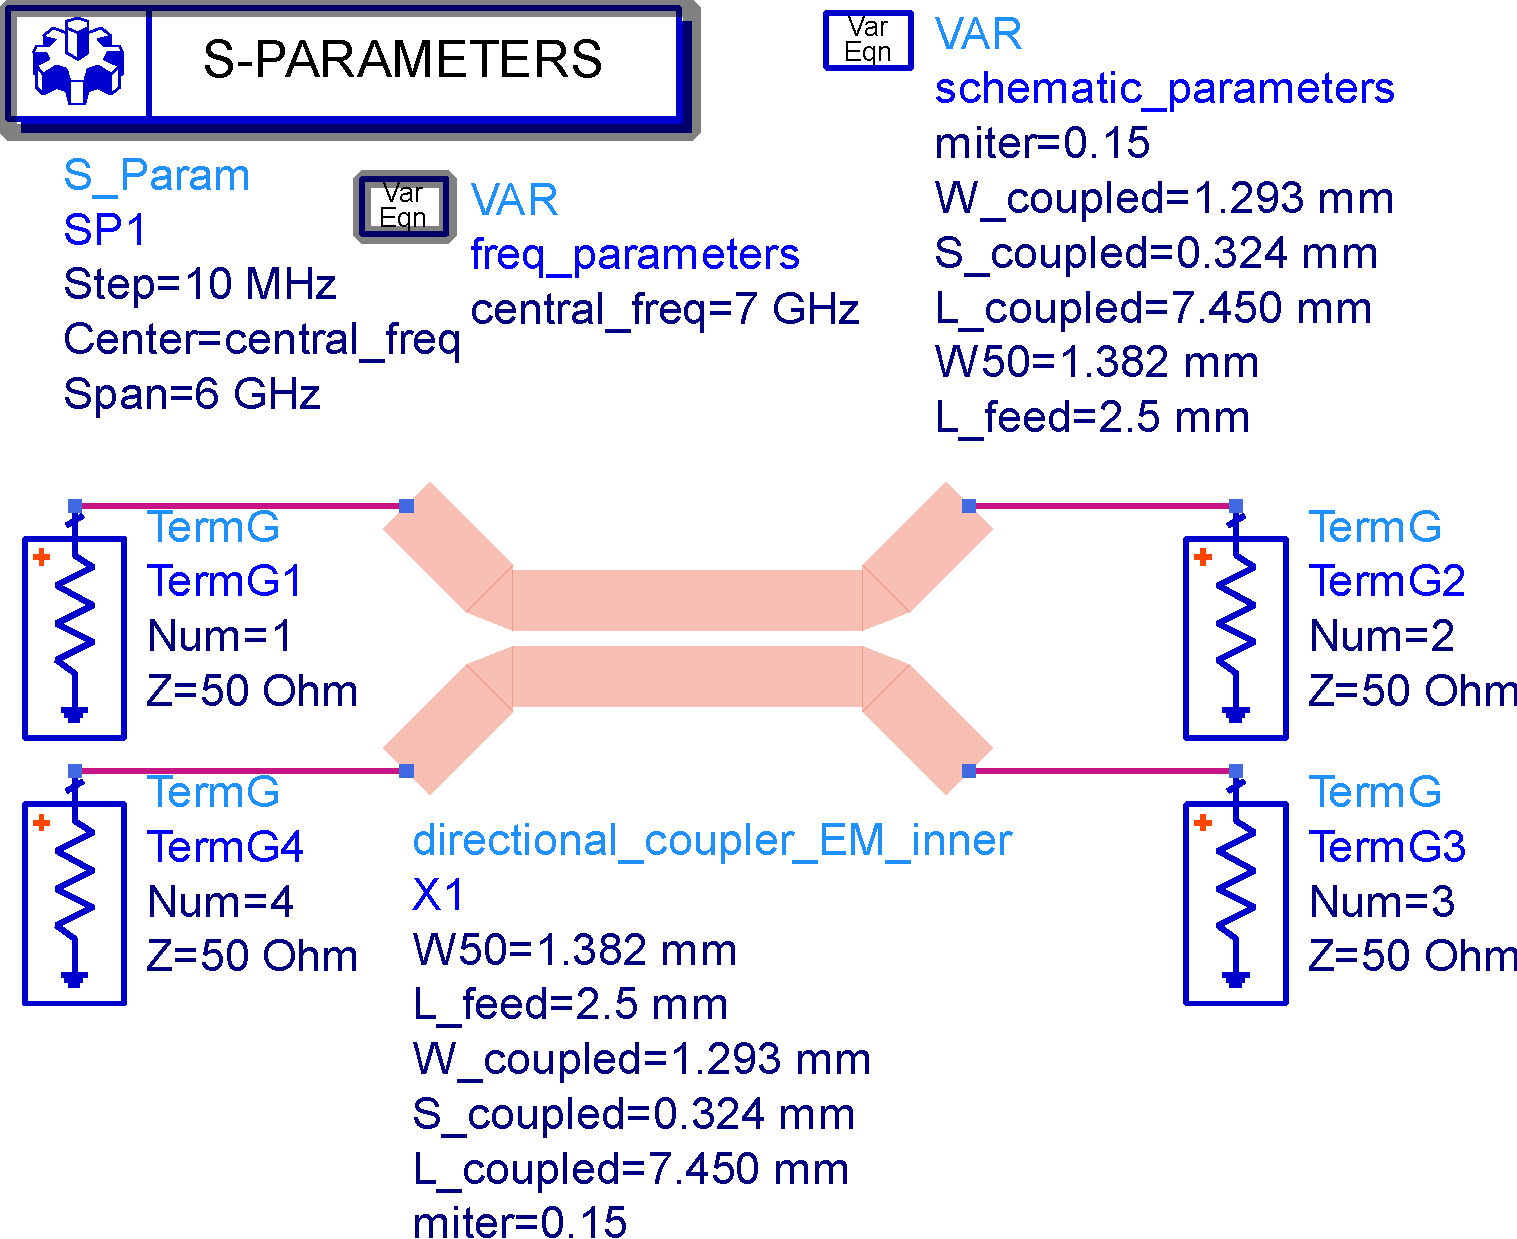
\includegraphics[width=0.8\textwidth]{directional_coupler_EM_schematic_2.pdf}
    \caption{Итоговый вид схемы}
    \label{fig:directional_coupler_EM_schematic_2}
\end{figure}

Запустим моделирование и отобразим частотные характеристики (Рис. \ref{fig:directional_coupler_EM_data_1}).

\begin{figure}[!ht]
    \centering
    \begin{subfigure}[b]{0.45\textwidth}
        \centering
        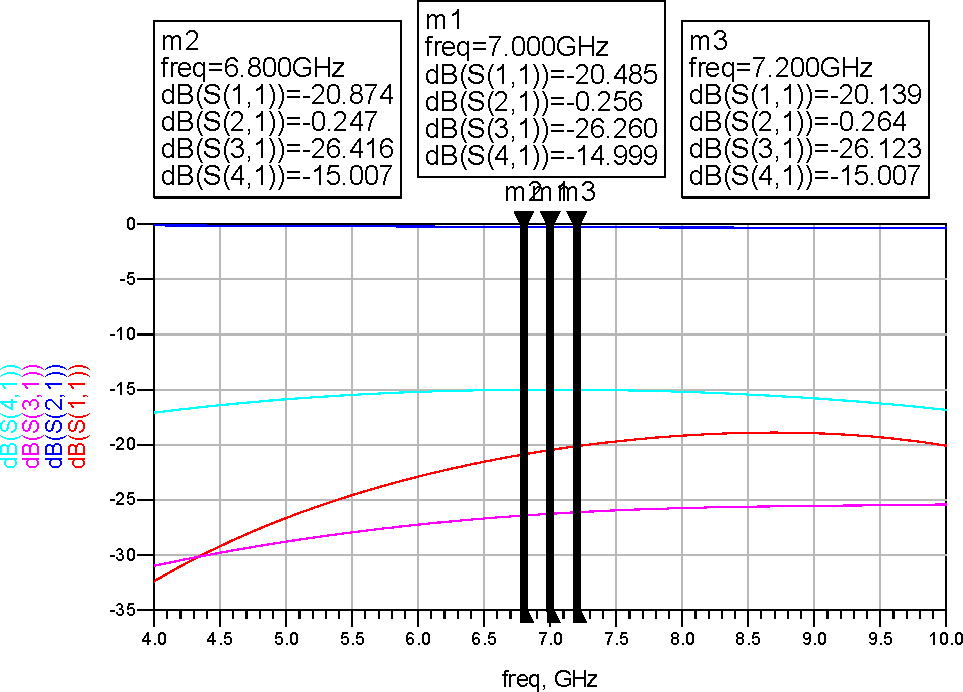
\includegraphics[width=\textwidth]{directional_coupler_EM_data_1_freq_response.pdf}
        \caption{}
        \label{fig:directional_coupler_EM_data_1_freq_response}
    \end{subfigure}
    \hfill
    \begin{subfigure}[b]{0.45\textwidth}
        \centering
        \includegraphics[width=\textwidth]{directional_coupler_EM_data_1_phase_response.pdf}
        \caption{}
        \label{fig:directional_coupler_EM_data_1_phase_response}
    \end{subfigure}
    \caption{
        Частотные характеристики моделируемой схемы в топологическом представлении:
        а) АЧХ;
        б) ФЧХ
    }
    \label{fig:directional_coupler_EM_data_1}
\end{figure}

